% !Mode:: "TeX:UTF-8" 



\BiSection{2.27}{Figures}

\fancyhead[R]{本题2.27由QC.Z完成}



解:

由$I_D=I_0e^{\frac{V_{GS}}{\xi V_T}}$得

$I_{D1}=I_0e^{\frac{V_{GS1}}{\xi V_T}}$

$I_{D2}=I_0e^{\frac{V_{GS2}}{\xi V_T}}$

上两式相除得

$\frac{I_{D2}}{I_{D1}}=\frac{I_0e^{\frac{V_{GS2}}{\xi V_T}}}{I_0e^{\frac{V_{GS1}}{\xi V_T}}}=e^{\frac{V_{GS2}-V_{GS1}}{\xi V_T}}=e^{\frac{\Delta V_{GS}}{\xi V_T}}$

假设$I_D$变化一个数量级($\frac{I_{D2}}{I_{D1}}=10$)有

$10=e^{\frac{\Delta V_{GS}}{\xi V_T}}$

$ln10=lne^{\frac{\Delta V_{GS}}{\xi V_T}}$

$ln10=\frac{\Delta V_{GS}}{\xi V_T}$

$\Delta V_{GS}=\xi V_Tln10$

$\Delta V_{GS}=\xi (\frac{kT}{q})ln10$

\begin{figure}[H] %H为当前位置,!htb为忽略美学标准,htbp为浮动图形
	\begin{minipage}{\linewidth}
		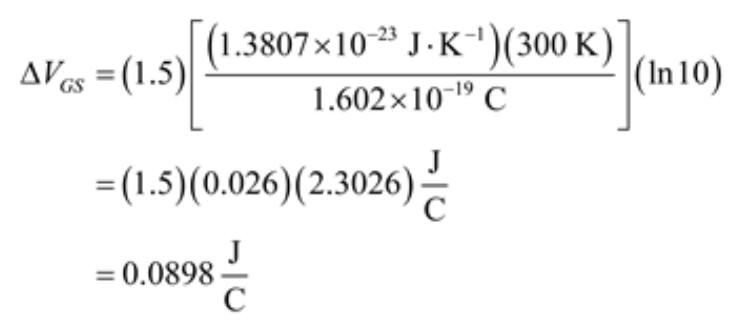
\includegraphics[width=1\linewidth]{2.27-1}
	\end{minipage}
\end{figure}

用$V$替换$\frac{J}{C}$





\begin{figure}[H] %H为当前位置,!htb为忽略美学标准,htbp为浮动图形
	\begin{minipage}{\linewidth}
		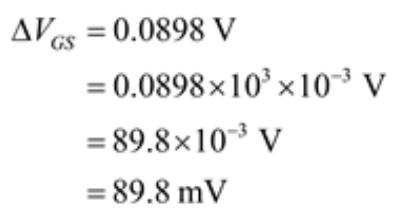
\includegraphics{2.27-2}
	\end{minipage}
\end{figure}









$g_m=\frac{I_D}{\xi V_T}=\frac{I_D}{\xi (\frac{kT}{q})}=\frac{qI_D}{\xi kT}$


\begin{figure}[H] %H为当前位置,!htb为忽略美学标准,htbp为浮动图形
	\begin{minipage}{\linewidth}
		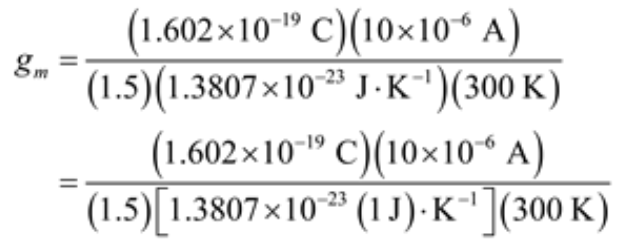
\includegraphics{2.27-3}
	\end{minipage}
\end{figure}



用$C\cdot J$替换$J$

\begin{figure}[H] %H为当前位置,!htb为忽略美学标准,htbp为浮动图形
	\begin{minipage}{\linewidth}
		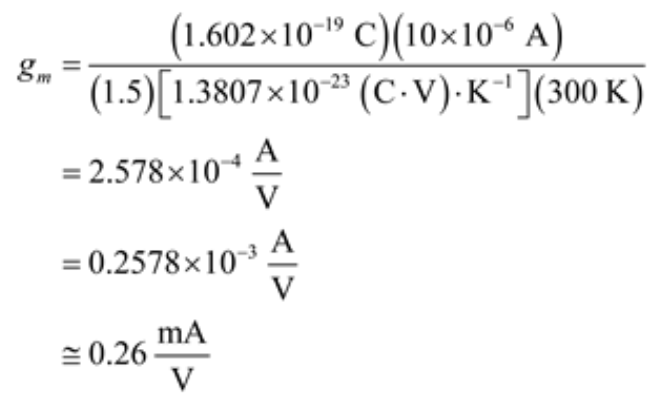
\includegraphics{2.27-4}
	\end{minipage}
\end{figure}














